\documentclass[12pt]{standalone}
\usepackage{subcaption}
\usepackage{tikz}

\begin{document}
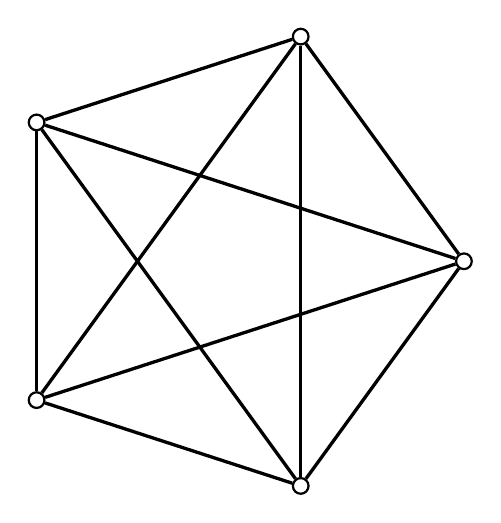
\begin{tikzpicture}[scale=1.5]
    \node[circle, thick, draw, inner sep=2pt] (a) at (0:2) {};
    \node[circle, thick, draw, inner sep=2pt] (b) at (72:2) {};
    \node[circle, thick, draw, inner sep=2pt] (c) at (144:2) {};
    \node[circle, thick, draw, inner sep=2pt] (d) at (216:2) {};
    \node[circle, thick, draw, inner sep=2pt] (e) at (288:2) {};
    \draw[very thick, black] (a) -- (b);
    \draw[very thick, black] (a) -- (c);
    \draw[very thick, black] (a) -- (d);
    \draw[very thick, black] (a) -- (e);
    \draw[very thick, black] (b) -- (c);
    \draw[very thick, black] (b) -- (d);
    \draw[very thick, black] (b) -- (e);
    \draw[very thick, black] (c) -- (d);
    \draw[very thick, black] (c) -- (e);
    \draw[very thick, black] (d) -- (e);
\end{tikzpicture}
\hspace{40pt}
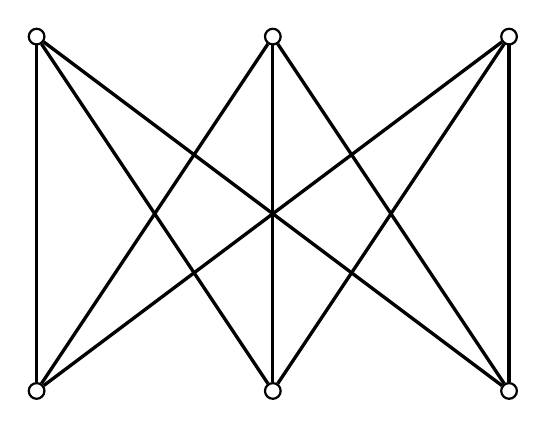
\begin{tikzpicture}[scale=1.5]
    \node[circle, thick, draw, inner sep=2pt] (a1) at (0,0) {};
    \node[circle, thick, draw, inner sep=2pt] (a2) at (2,0) {};
    \node[circle, thick, draw, inner sep=2pt] (a3) at (-2,0) {};
    \node[circle, thick, draw, inner sep=2pt] (b1) at (0,3) {};
    \node[circle, thick, draw, inner sep=2pt] (b2) at (2,3) {};
    \node[circle, thick, draw, inner sep=2pt] (b3) at (-2,3) {};
    \draw[very thick, black] (a1) -- (b1);
    \draw[very thick, black] (a1) -- (b2);
    \draw[very thick, black] (a1) -- (b3);
    \draw[very thick, black] (a2) -- (b1);
    \draw[very thick, black] (a2) -- (b2);
    \draw[very thick, black] (a2) -- (b3);
    \draw[very thick, black] (a3) -- (b1);
    \draw[very thick, black] (a3) -- (b2);
    \draw[very thick, black] (a3) -- (b3);
\end{tikzpicture}
\end{document}
